\documentclass[11pt,a4paper]{article}
\usepackage[utf8]{inputenc}
\usepackage[T1]{fontenc}
\usepackage{graphicx}
\usepackage{booktabs}
\usepackage{longtable}
\usepackage{array}
\usepackage[hidelinks]{hyperref}
\usepackage[margin=2.5cm]{geometry}
\usepackage{microtype}
\graphicspath{{figures/}}
\title{Ontology Drift in Cyber Threat Intelligence:\\
A Longitudinal Measurement of MITRE ATT\&CK and a Reporting Contract\\
for Reproducible CTI Analytics}
\date{}
\begin{document}
\maketitle

\begin{abstract}


Security machine learning spent a decade learning to control for bias in its data. All of that discipline assumes something it never states: that the label space is fixed. In cyber threat intelligence it is not. MITRE ATT\&CK is the instrument in which coverage, attribution and benchmark labels are denominated, and it has been re-issued 109 times across three domains since January 2018 without any downstream result recording which issue it used. From a longitudinal database of 106 domain-release pairs we measure four drift processes separately, then run controlled experiments holding the adversary intelligence fixed while only the vocabulary moves. MITRE's Enterprise identifier accounting is complete — every revoked technique carries exactly one successor edge and none dangle — and post-2020 identifier survival to the newest release never falls below 0.970. Yet 0.749 of the identifier-stable techniques of v7.0 have edited descriptions by v19.0, ATT\&CK's own version field detects a rewrite at precision 0.447 and recall 0.641, 0.323 of new group-technique edges for pre-existing groups are bookkeeping rather than intelligence, and a frozen capability that claimed 97.0\% coverage reads 17.4\% at v19.0. Vocabulary mismatch alone changes the named threat actor in 0.722 of pre-restructuring observations and still in 0.022 across one modern release boundary, concentrated on exactly the groups that are identifiable at all. Normalization recovers 0.42 to 0.53 of the legacy penalty, almost nothing modern, and nothing semantic, so the contribution is a reporting contract rather than a crosswalk.

\end{abstract}
\section{Introduction}

A coverage percentage, an attribution verdict and a benchmark score are measurements, and every measurement is stated in units. In cyber threat intelligence the unit is the ATT\&CK technique identifier, and the number means something only relative to the edition of the catalogue supplying both the numerator's vocabulary and the denominator's cardinality [63, 74]. Between an attribution system published in 2019 and a successor published in 2023 that beats it on the same corpus, the label space lost roughly half its identifiers in one release, gained a level of abstraction that did not previously exist, and rewrote three-quarters of the descriptions of the terms that survived. Neither paper declares its release; no venue asks. Those two numbers are readings from different instruments, reported in the same units by convention alone.

Security machine learning knows this class of error: TESSERACT gave the field a vocabulary for temporal and spatial bias [67], Arp et al. catalogued ten recurring methodological failures [35], and drift detection and conformal rejection carried the concern into deployment [22, 70]. Every one of those instruments assumes a fixed label space — dataset-shift taxonomy holds the class set constant [33], class-incremental learning handles only the additive quadrant [24], evolving-class-ontology work only relabelling [43] — while ATT\&CK performs addition, deprecation, revocation, re-cutting, cross-layer promotion and silent redefinition. Concept drift moves the data under a fixed ruler; ontology drift moves the ruler, and a model perfectly robust to the first still reports an incomparable number under the second.

We argue by measurement and make the concessions the measurement forces. The apparatus is real: pinning a release is MITRE's documented first-class workflow, tombstones are guaranteed, revocation edges are typed, and a change-computation tool ships with an explicit class for objects patched without a version increment [1, 7, 34, 48], so anyone holding that documentation refutes a naive version of this paper in a paragraph. The noise floor is real: products pinned to one release disagree about the label for the same behaviour [74] and roughly a third of ATT\&CK groups have any technique unique to them [59]; we do not claim drift dominates that noise, only that it is separable by construction, and we test additivity rather than assuming it (Section 7.3). The remedy is weak: normalization is worth tens of points on pre-2020 artefacts and under one point on modern ones, with an interval spanning zero in most modern conditions (Section 8).

Four contributions follow: a longitudinal measurement of drift over every public release of all three domains, decomposed into processes that behave differently in time (Section 6); controlled experiments on attribution, coverage, mitigation ranking and benchmark label validity in which only the vocabulary moves (Sections 7 and 9); a decomposition of apparent knowledge growth into intelligence and bookkeeping (Section 6.4); and a normalization protocol whose measured limits are themselves the result (Section 8), with the reporting discipline that follows (Section 10). The problem is current, not historical: four months before this analysis, ATT\&CK v19 retired Defense Evasion as a tactic, renamed TA0005 in place to Stealth, minted TA0112 Defense Impairment, and revoked the twelve-child T1562 family into the new arrangement [78].

\end{abstract}
\section{Background: ATT\&CK as a Versioned Ontology}

ATT\&CK organises adversary behaviour into tactics, techniques and sub-techniques and links them to intrusion sets, software, mitigations and data components. Its design documentation states that inclusion criteria are non-stationary and that the abstraction level of a technique is an editorial choice rather than a natural kind [14]. Practitioners defending its structure describe it as an ontology rather than a taxonomy [77], which places it inside a literature where change management is the core task of both versioning and evolution [56].

That literature supplies the yardstick. OBO Foundry requires version IRIs, release immutability and perpetual resolvability [55], mandates identifier uniqueness and forbids reuse [53], and requires in its term-stability principle that the referent of an identifier not change, separating exact from inexact successors and making obsoletion visible in the human-readable label [54]. OWL has supplied \texttt{versionIRI}, \texttt{priorVersion}, \texttt{backwardCompatibleWith} and \texttt{owl:deprecated} for two decades [57], and COnto-Diff types complex change operations as evolution mappings rather than untyped diffs [26]. Biomedicine demonstrated the downstream consequence: Gene Ontology evolution changes the interpretation of analyses computed over it, so a conclusion moves with no new experiment [69]. Security vocabularies have their own instances, in CVE lifecycle states [31], CVE-to-CWE-to-CPE abstraction-ladder instability [32], CVSS fragmentation across versions [39], and knowledge-graph work tracking vocabulary churn and instance usage as separate time series [37].

Measured against that yardstick ATT\&CK scores well on some axes and has nothing on others. Releases are immutable and addressable [1, 55], and retirement is typed and non-destructive: an object with a successor is revoked and carries a \texttt{revoked-by} edge, one without is deprecated, and both are retained so dependent workflows do not break [1]. The Center for Threat-Informed Defense funds ATT\&CK Sync to flag mappings affected by a release [5], an institutional concession that staying in sync is an operational burden, and the Navigator layer format can record the content version of a coverage layer [15], though the field is optional and defaults silently to current [16] and widely used tooling omits it altogether [79]. What ATT\&CK lacks is the inexact-successor relation, a controlled obsolescence-reason vocabulary, label-level visibility of obsoletion, prior-version and compatibility links, and a typed evolution mapping published as an artefact in its own right. Sections 6 and 8 price each absence. One structural fact shapes everything downstream: the March 2020 introduction of sub-techniques was not an addition but a re-cut, it is the most-cited instability in the ATT\&CK literature [47, 63], and Section 6.5 shows it is one draw from a live hazard rather than a closed wound.

\end{abstract}
\section{Related Work}

Four literatures bear on this problem and none of them measures it.

\textbf{CTI quality.} A mature line defines quality dimensions and builds instruments to score feeds against them: accuracy, completeness, timeliness, relevance, provenance and interoperability recur across the canonical treatments [60, 76], with dynamic assessment and weighted criteria added later [27], feed evaluations establishing that public feeds overlap little and age badly [41, 45], practitioner quality assurance studied directly [40], community feeds metered [38], a 2025 measurement-based survey consolidating the field [11], and separate complaints about exchange-format validity [83] and vulnerability-database quality [25]. None of these frameworks names the reference vocabulary's edition as a dimension. This is an audited absence and we state its bound: across the sources reachable in this environment we found no such dimension defined, and we lacked full text for some, so we claim the absence of a named dimension rather than the absence of any awareness.

\textbf{ATT\&CK-based analytics.} The systematization of ATT\&CK establishes that coverage claims are not comparable across products and flags temporal instability as open [63]; a 2025 survey sets the bar a contribution must clear [47]. Virkud et al. demonstrate non-comparability at a single pinned release: rules from different vendors describing the same behaviour carry disjoint labels, and recomputing coverage from raw artefacts collapses the differences between products [74]. Shen et al. argue per-technique tallies are the wrong unit [62]; MITRE's Evaluations refuse to emit a coverage score [46]; practitioners are blunter, that a heatmap counts rules rather than coverage, that a 100\% claim is a red flag, that several incompatible denominators circulate, and that layers are built ad hoc over a versioned data-source mapping [80, 81, 82, 84]. Summiting the Pyramid replaces techniques with implementations as the denominator outright [64], and mitigation coverage has a ceiling set by the control catalogue rather than the product [58]. All of this establishes disagreement at one version; none of it measures what a version change costs.

\textbf{Extraction, benchmarks and attribution.} The extraction line runs from TTPDrill [71] through rcATT [44] to TTPHunter and its successor [72], with graph-based systems alongside [2] and recent multi-label work declining to treat existing annotations as gold [52, 73]. LLM-era benchmarks are the dominant evaluation surface: CTIBench treats authoritative sources as fixed and time-controls one task but not the ATT\&CK task [30]; a successor line grew from 691 to 1,860 QA pairs under one identifier and the same nine-task taxonomy [29]; AthenaBench argues static benchmarks go stale and proposes live-API construction [13]; large instruction corpora span two decades of reports with no declared release [61]; synthesis work targets the long tail [65]; sequence-level benchmarks add tactic ordering as a drift surface [17]; telemetry grounding is the only structurally drift-resistant design in the set [28]; and answer-key decay has been quantified outside security [75]. Attribution has moved to TTP sequences [23] and is surveyed by artefact type rather than ontology version [12], while two results bound what it can do at all: most ATT\&CK groups have no group-specific behaviour [59], and LLM agents reproduce documented APT profiles at 55-80\% precision [66]. Extractor errors concentrate among same-tactic, description-overlapping techniques [20], and vendor fragmentation compounds all of it [68]. The common feature, as Section 9 shows, is that the gold label space is a file whose provenance is undeclared [3, 6].

\textbf{Concept drift in security ML.} Dataset-shift taxonomies are formulated over a fixed label space [33]; TESSERACT establishes temporal hygiene [67]; CADE explains drifting samples [22]; conformal evaluation rejects under drift [70]; adaptation work assumes a fixed vocabulary while the distribution moves [50]; and the catalogue of security-ML pitfalls has no entry for a label space that changes between training and evaluation [35]. Where the label space does change, the machinery is class-incremental learning [24] and continual learning with evolving class ontologies [43], the closest security instance is MOTIF's unstable family set [51], and AVClass is the prior art for alias resolution as a published normalization artefact [19]. IncreTTP is, as far as we found, the only work framing ATT\&CK version updates as concept drift, and its remedy is incremental learning rather than measurement [42]. The boundary is the contribution point: concept drift is change in the conditional distribution with the label set fixed; ontology drift is change in the set itself and in what its members mean [21].

\end{abstract}
\section{Problem Formalization and Drift Taxonomy}

Let a release \texttt{V} of an ATT\&CK domain determine a label space \texttt{L\_V} of live technique identifiers together with an intension map \texttt{ι\_V} sending each identifier to what defines it: description, detection guidance, tactic assignment, platforms. A CTI artefact is a pair \texttt{(A, V)} with \texttt{A ⊆ L\_V}. In deployed practice \texttt{V} is almost never recorded (Table 12), so what circulates is \texttt{A} alone. Two artefacts are comparable when expressed in the same label space under the same intension map — not a strong requirement, simply the ordinary requirement that measurements reported in the same units be reported in the same units.

Six operators carry \texttt{(L\_V, ι\_V)} to \texttt{(L\_W, ι\_W)}. \textbf{O1 Addition}: a new identifier with no predecessor, the only operator class-incremental learning handles [24] and the only one benign for backward comparison; forward it is not benign, because a growing denominator makes a frozen capability's percentage fall with no change in the capability (Table 8). \textbf{O2 Deprecation}: withdrawn with no successor, marked and retained [1]. \textbf{O3 Revocation with a typed successor}: the well-handled case on which the ecosystem's defence rests, and in our corpus every revoked Enterprise identifier resolves to a live one (Table 3). \textbf{O4 Re-cut}: a concept split across successors, or several merged into one. Because \texttt{revoked-by} is a function and never one-to-many, a split is representable only as merges onto the narrowest survivor. It is not true that the relation cannot express the v19 re-cut; it can, as merges. The defect is annotation rather than expressiveness — the merge is unlabelled, so a consumer applying the crosswalk mechanically cannot distinguish an exact successor from a narrowing, which ontology engineering settled by splitting the successor relation into exact and inexact variants [54] and typing complex change operations [26, 56]. \textbf{O5 Cross-layer reassignment}: a technique demoted onto a sub-technique, a sub-technique promoted, or a technique promoted to a tactic; the crosswalk carries no abstraction-level annotation, and a promotion to the tactic layer is not representable at all, since \texttt{revoked-by} cannot point a technique at a tactic and no tactic object in the corpus carries a revocation edge. \textbf{O6 Intensional rewriting}: the identifier survives and what it denotes moves, invisible to every identifier-based mechanism in the ecosystem.

O1 to O5 are referential; O6 is intensional, and that split organises the paper because the two components have different dynamics, different downstream consequences and different repair prospects. Cutting across it is a distinction we consider more practically important. Call an operator signalled if the published artefact carries a machine-readable marker a consumer can test. O2 and O3 are signalled; O4 and O5 are partially signalled, since the edges exist but carry no type, so a consumer learns that something changed and not what; O6 is unsignalled, because its only candidate marker, the object version field, operates at precision 0.447 and recall 0.641 (Section 6.3). The component of drift that is well handled is the component everybody points at, and the component that is not handled at all is the component nobody can see.

Two artefacts are version-comparable when both have been projected onto one reference release and the projection's residual is declared. Projection is transitive closure over the retirement relation; it is a function and not an injection, so it can merge and land on a different abstraction level, and its residual is the four-way ledger of kept, merged, demoted and dropped. A protocol returning only the projected set destroys exactly the information a reader needs to judge comparability (Section 8). Ontology drift accordingly damages construct validity, because after O6 the construct measured is not the construct the labels name; internal validity, because after O4 or O5 measured profile breadth falls with no change in the intelligence; external validity, because after O1 an unchanged capability reports a falling number; and conclusion validity, which Section 7 shows reaches the named actor, the top-ranked mitigation and the pass/fail verdict. Because a study of drift is exposed to its own subject, we commit in advance to four requirements and audit them in Section 11: \textbf{R1}, the contrast holds everything constant except the vocabulary; \textbf{R2}, a stated noise model, since holding a nuisance term at zero establishes separability and says nothing about additivity; \textbf{R3}, a declared closure boundary; \textbf{R4}, a named falsifier.

\end{abstract}
\section{Data and Methodology}

We clone MITRE's \texttt{attack-stix-data} repository, which publishes every release as an immutable STIX 2.1 bundle at a stable path [1]. Its index enumerates 109 versioned bundle entries, 41 Enterprise, 41 Mobile and 27 ICS; our extraction materialises 106 domain-release pairs, 41 Enterprise, 38 Mobile and 27 ICS. The three-entry difference falls entirely at Mobile v11.0 to v11.2, pre-release entries the published sequence skips as it steps from v10.1 to v11.3, which we exclude. We report both counts rather than quietly adopting the convenient one, because undeclared denominators are how measurements go wrong. Each bundle is parsed into a relational store holding every object's identifiers, flags, \texttt{x\_mitre\_version}, timestamps, kill-chain phases, platforms, and the text and SHA-256 digests of the description and detection fields, with every typed relationship. Release-level analyses use major releases only — the \texttt{.0} release of each major version, or the earliest available — giving 19 Enterprise, 19 Mobile and 12 ICS analysis points, because patch releases are irregular in cadence and scope and mixing them in would make a per-release transition mean different things in different eras. Section 9 deliberately does the opposite and uses every published release, since there the question is which release a label file could have been written against.

\textbf{Table 1.} The release corpus. Major releases are the analysis points for churn, survival and drift; all releases are used for the label-validity analysis of Section 9.

\begin{center}\footnotesize
\begin{tabular}{llll}
\toprule
Domain & Releases analysed (major / all) & First & Last \\
\midrule
Enterprise & 19 / 41 & v1.0 (2018-01-17) & v19.0 (2026-04-28) \\
Mobile & 19 / 38 & v1.0 (2018-01-17) & v19.0 (2026-04-28) \\
Ics & 12 / 27 & v8.0 (2020-10-27) & v19.0 (2026-04-28) \\
\bottomrule
\end{tabular}
\end{center}

The live set is the \texttt{attack-pattern} objects with both retirement flags false, and it is the denominator of every coverage claim. Identifier Jaccard is computed over consecutive majors with a revoked identifier treated as absent, since it is unusable as a label even though the object is retained. An identifier is recoverable at a target if transitive \texttt{revoked-by} closure from it, cycle-safe and bounded at ten hops, terminates in the live set. Semantic drift is measured on identifier-stable techniques only: an edit is inequality of description digests, similarity is the Jaccard index over lowercased alphanumeric token sets, and a substantial rewrite is similarity below 0.8, a convention reported alongside the full mean-similarity series. Bag-of-words similarity is deliberately crude: monotone in shared vocabulary, model-free, and incapable of importing an embedding's own drift into a measurement of drift. Growth decomposition assigns each newly added group-technique edge to one cause in a fixed order — new actor, revocation re-mapping, sub-technique refinement, new technique, genuine new intelligence — with re-mapping tested before refinement so an ambiguous edge is charged to bookkeeping.

Four experiments share one principle, satisfying R1: the intelligence is held fixed and only the vocabulary varies. \textbf{Attribution.} The analysis release is v19.0. Modern group profiles are back-projected into a legacy vocabulary by a map built once per pair: a modern technique maps to itself if live then, else to the pre-revocation identifier resolving onto it, else to the nearest live ancestor within five hops, else it is dropped as a behaviour with no expression in that era. Each of 500 trials samples a group, draws k = 10 techniques from its modern profile, and scores four conditions over identical draws — back-projected (labelled contemporaneous in the released results files), naive, ATT\&CK-Norm, oracle. Scoring is IDF-weighted cosine; the drift penalty is back-projected minus naive top-1 accuracy; recovery is the share of that penalty normalization returns; intervals are paired bootstrap with 2,000 resamples, and robustness sweeps three scorers and two profile definitions (Table 7). \textbf{Coverage.} A capability is frozen at a release as the techniques reachable by \texttt{mitigates} edges there, then re-measured at v19.0 naively and after normalization, with a 500-sample random-portfolio sweep and a prevalence-weighted variant. \textbf{Conclusion instability.} The same machinery is read out at verdict level and as Kendall tau over mitigation rankings. \textbf{Label validity.} Four deployed corpora are parsed from their own label files rather than their papers, every identifier is checked for liveness at every published release, and the provenance interval is the set of releases at which every identifier is simultaneously live — an empty interval meaning the artefact mixes mutually exclusive vocabularies.

Every number in Sections 6 to 9 is produced by scripts in \texttt{code/} from public bundles and label files, runs end to end from one shell script, and is written to JSON from which the tables are generated rather than transcribed. Three evidence tiers are marked throughout: Tier A, our own measurement and artefacts read in full from local clones; Tier B, secondary literature reachable here only through search summaries, attributed as reported and never quoted; Tier C, an audited absence, stated with the bound of the search that found it.

\end{abstract}
\section{Measuring Ontology Drift in ATT\&CK}

\subsection{6.1 Two clocks, not one}

\textbf{Figure 1.} Live technique count across Enterprise releases, with per-release additions, revocations and description rewrites on a shared time axis.

\begin{figure}[htbp]
\centering
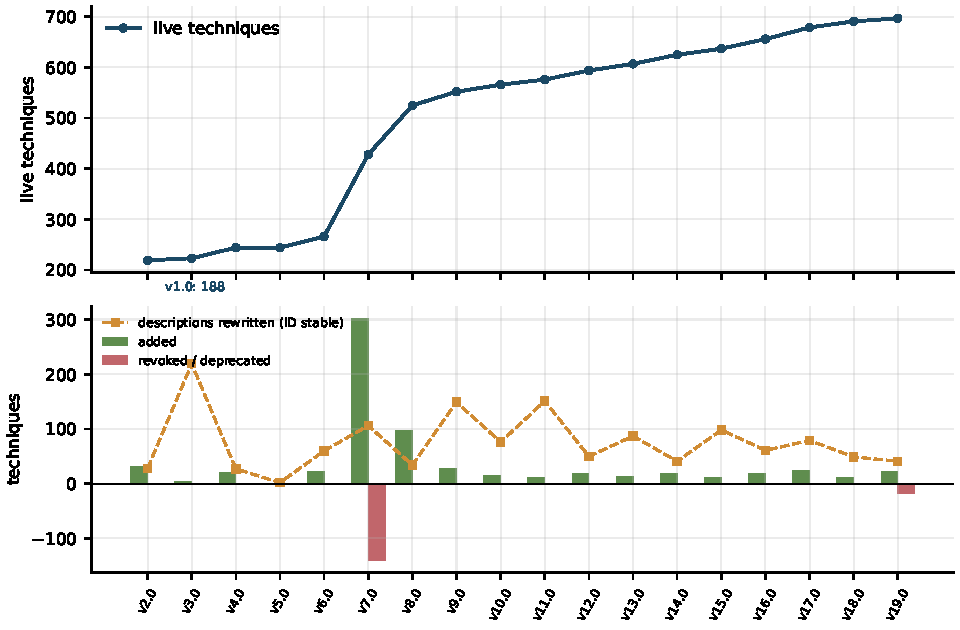
\includegraphics[width=\linewidth]{fig1_growth_churn.pdf}
\caption{Live technique count per Enterprise release, and per-release additions, retirements and description rewrites.}
\label{fig:1}
\end{figure}


\textbf{Table 2.} Per-release Enterprise churn across consecutive major releases. Rewrite and tactic columns count only techniques live in both releases; \texttt{J(ID)} is the identifier Jaccard; edges are group-to-technique \texttt{uses} edges.

\begin{center}\footnotesize
\begin{tabular}{llllllllllll}
\toprule
Transition & Date & Live & Added & Revoked & Deprecated & Renamed & Desc. rewritten & Detection rewritten & Tactic changed & J(ID) & Edges +/- \\
\midrule
v1.0→v2.0 & 2018-04-18 & 219 & 31 & 0 & 0 & 2 & 28 & 0 & 5 & 0.858 & +135/−0 \\
v2.0→v3.0 & 2018-10-23 & 223 & 4 & 0 & 0 & 1 & 219 & 218 & 4 & 0.982 & +285/−0 \\
v3.0→v4.0 & 2019-04-30 & 244 & 21 & 0 & 0 & 1 & 27 & 10 & 1 & 0.914 & +237/−2 \\
v4.0→v5.0 & 2019-07-19 & 244 & 0 & 0 & 0 & 0 & 2 & 0 & 0 & 1.000 & +100/−0 \\
v5.0→v6.0 & 2019-10-23 & 266 & 22 & 0 & 0 & 2 & 60 & 24 & 2 & 0.917 & +102/−0 \\
v6.0→v7.0 & 2020-03-31 & 428 & 302 & 129 & 11 & 17 & 106 & 60 & 10 & 0.222 & +1235/−750 \\
v7.0→v8.0 & 2020-10-27 & 525 & 97 & 0 & 0 & 3 & 34 & 17 & 0 & 0.815 & +102/−2 \\
v8.0→v9.0 & 2021-04-29 & 552 & 27 & 0 & 0 & 6 & 149 & 52 & 5 & 0.951 & +642/−2 \\
v9.0→v10.0 & 2021-10-21 & 566 & 15 & 0 & 1 & 2 & 76 & 66 & 0 & 0.972 & +312/−1 \\
v10.0→v11.0 & 2022-04-25 & 576 & 12 & 2 & 0 & 9 & 151 & 44 & 0 & 0.976 & +288/−1 \\
v11.0→v12.0 & 2022-10-25 & 594 & 18 & 0 & 0 & 2 & 50 & 0 & 0 & 0.970 & +252/−0 \\
v12.0→v13.0 & 2023-04-25 & 607 & 13 & 0 & 0 & 1 & 87 & 13 & 0 & 0.979 & +112/−16 \\
v13.0→v14.0 & 2023-10-31 & 625 & 18 & 0 & 0 & 1 & 41 & 2 & 6 & 0.971 & +178/−1 \\
v14.0→v15.0 & 2024-04-23 & 637 & 12 & 0 & 0 & 3 & 98 & 4 & 0 & 0.981 & +208/−34 \\
v15.0→v16.0 & 2024-10-31 & 656 & 19 & 0 & 0 & 1 & 61 & 0 & 0 & 0.971 & +417/−14 \\
v16.0→v17.0 & 2025-04-22 & 679 & 24 & 1 & 0 & 5 & 79 & 5 & 2 & 0.963 & +313/−558 \\
v17.0→v18.0 & 2025-10-28 & 691 & 12 & 0 & 0 & 2 & 49 & 583 & 0 & 0.983 & +328/−11 \\
v18.0→v19.0 & 2026-04-28 & 697 & 23 & 17 & 0 & 4 & 41 & 0 & 198 & 0.944 & +270/−86 \\
\bottomrule
\end{tabular}
\end{center}

Read the identifier column alone and the episodic reading is irresistible: one transition, v6.0 to v7.0, has an identifier Jaccard of 0.222, adds 302 techniques, revokes 129, deprecates 11, and rewrites the group-technique graph by removing 750 edges and adding 1,235. The next largest drop in eight years is 0.944, at the most recent transition. Read any other column and that reading collapses. Description rewrites among surviving techniques never fall below 27 and reach 151 at v10.0 to v11.0, whose identifier Jaccard is 0.976. Detection rewrites are burstier: 583 of 691 surviving techniques had their detection guidance rewritten between v17.0 and v18.0, a transition any identifier-keyed diff reports as one of the quietest in ATT\&CK's history. The tactic column, empty or near-empty for sixteen transitions, reads 198 at the most recent. This is the two-clock structure, and stating it precisely is the first result: a slow episodic referential clock and a fast continuous intensional clock, so that any risk statement reporting one without the other is wrong by a factor that depends on which column the reader happened to look at.

\subsection{6.2 Survival: the concession, measured}

\textbf{Figure 2.} Identifier survival curves by source release to v19.0, with the recoverable fraction under transitive \texttt{revoked-by} closure overlaid.

\begin{figure}[htbp]
\centering
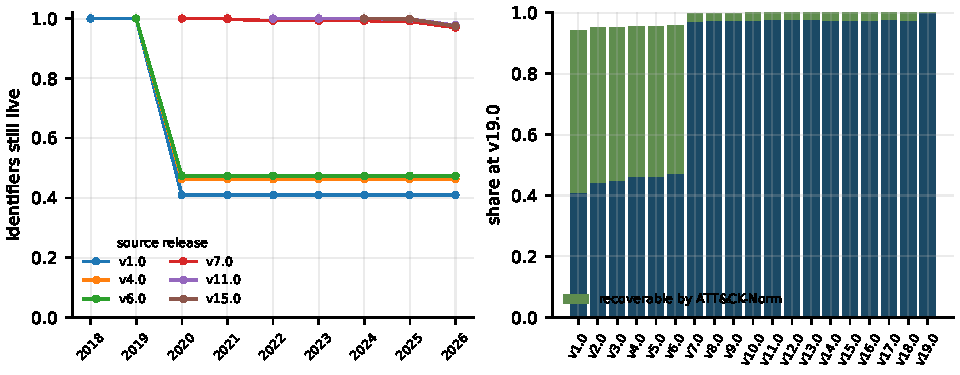
\includegraphics[width=\linewidth]{fig2_survival.pdf}
\caption{Identifier survival by source release, and the share recoverable through the published revocation graph at the newest release.}
\label{fig:2}
\end{figure}


\textbf{Table 3.} Identifier survival to v19.0 by source release. Recoverable counts revoked or absent identifiers whose transitive closure terminates at a live identifier.

\begin{center}\footnotesize
\begin{tabular}{lllllllll}
\toprule
Source release & Date & Identifiers & Live at v19.0 & Survival & Revoked & Deprecated & Recoverable & Half-life \\
\midrule
v1.0 & 2018-01-17 & 188 & 77 & 0.410 & 100 & 11 & 100 & v7.0 (2.2 y) \\
v2.0 & 2018-04-18 & 219 & 97 & 0.443 & 111 & 11 & 111 & v7.0 (2.0 y) \\
v3.0 & 2018-10-23 & 223 & 100 & 0.448 & 112 & 11 & 112 & v7.0 (1.4 y) \\
v4.0 & 2019-04-30 & 244 & 113 & 0.463 & 120 & 11 & 120 & v7.0 (0.9 y) \\
v5.0 & 2019-07-19 & 244 & 113 & 0.463 & 120 & 11 & 120 & v7.0 (0.7 y) \\
v6.0 & 2019-10-23 & 266 & 126 & 0.474 & 129 & 11 & 129 & v7.0 (0.4 y) \\
v7.0 & 2020-03-31 & 428 & 415 & 0.970 & 12 & 1 & 12 & not reached \\
v8.0 & 2020-10-27 & 525 & 511 & 0.973 & 13 & 1 & 13 & not reached \\
v9.0 & 2021-04-29 & 552 & 538 & 0.975 & 13 & 1 & 13 & not reached \\
v10.0 & 2021-10-21 & 566 & 551 & 0.973 & 15 & 0 & 15 & not reached \\
v11.0 & 2022-04-25 & 576 & 563 & 0.977 & 13 & 0 & 13 & not reached \\
v12.0 & 2022-10-25 & 594 & 581 & 0.978 & 13 & 0 & 13 & not reached \\
v13.0 & 2023-04-25 & 607 & 593 & 0.977 & 14 & 0 & 14 & not reached \\
v14.0 & 2023-10-31 & 625 & 609 & 0.974 & 16 & 0 & 16 & not reached \\
v15.0 & 2024-04-23 & 637 & 621 & 0.975 & 16 & 0 & 16 & not reached \\
v16.0 & 2024-10-31 & 656 & 640 & 0.976 & 16 & 0 & 16 & not reached \\
v17.0 & 2025-04-22 & 679 & 663 & 0.976 & 16 & 0 & 16 & not reached \\
v18.0 & 2025-10-28 & 691 & 674 & 0.975 & 17 & 0 & 17 & not reached \\
v19.0 & 2026-04-28 & 697 & 697 & 1.000 & 0 & 0 & 0 & not reached \\
\bottomrule
\end{tabular}
\end{center}

The recoverable column equals the revoked column in every Enterprise row and the absent count is zero throughout. Recomputing from the v19.2 bundle gives 858 \texttt{attack-pattern} objects — 697 live, 149 revoked, 12 deprecated — and 149 \texttt{revoked-by} edges from 149 distinct sources. Every revoked Enterprise technique has exactly one successor and none dangle, and we concede this without qualification because conceding it is what makes the remaining argument non-trivial [1]. Each boundary of the concession is a finding. It is Enterprise-only: in Mobile, 34 survival rows record identifiers absent rather than tombstoned, and all 76 ATT\&CK identifiers of Mobile v1.0 are gone from v3.0 onward with no successor edge of any kind. The relation is never one-to-many, so a split appears only as merges onto whichever survivor the curator judges narrowest, with eight Enterprise targets absorbing 20 predecessors and the largest absorbing five. And retirement routinely crosses abstraction levels: of the 149 edges, 119 map a top-level technique onto a sub-technique, 13 top onto top, 10 sub onto sub, and 7 promote a sub-technique to a parent. A crosswalk that resolves in one hop, reports success, and silently narrows the extension of the original assertion is not broken; it is a 1:1 relation doing what a 1:1 relation can do in a situation that needs more [54].

The tactic layer has no retirement relation at all: across all three domains and every release our extraction finds 5,599 revocation edges and none involve a tactic object. Between v18.1 and v19.2 the object carrying TA0005 keeps its UUID and identifier while its name changes from Defense Evasion to Stealth, its shortname from \texttt{defense-evasion} to \texttt{stealth}, and its \texttt{x\_mitre\_version} stays at 1.0, with TA0112 Defense Impairment minted alongside and T1562 retired into the new arrangement [78]. Any analytic joining on TA0005 across that boundary compares two different concepts with no revocation, no version increment and nothing to follow. This is the edit that the stability principle exists to forbid: a changed referent requires a new identifier [54].

\subsection{6.3 Intensional drift, and why ATT\&CK cannot signal it}

\textbf{Figure 3.} Silent semantic drift among identifier-stable techniques: share with edited descriptions and share substantially rewritten, by source release, measured at v19.0.

\begin{figure}[htbp]
\centering
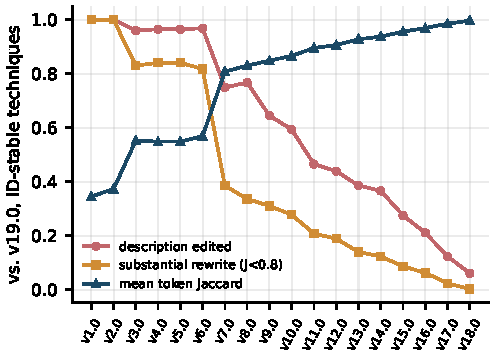
\includegraphics[width=\linewidth]{fig3_semantic_drift.pdf}
\caption{Silent semantic drift among techniques whose identifiers never changed.}
\label{fig:3}
\end{figure}


\textbf{Table 4.} Semantic drift among techniques live at both the source release and v19.0. Token Jaccard is over lowercased alphanumeric token sets of the description; a substantial rewrite is below 0.8.

\begin{center}\footnotesize
\begin{tabular}{lllll}
\toprule
Source release & ID-stable techniques & Description edited & Mean token Jaccard & Substantial rewrite (J<0.8) \\
\midrule
v1.0 & 77 & 1.000 & 0.345 & 1.000 \\
v2.0 & 97 & 1.000 & 0.373 & 1.000 \\
v3.0 & 100 & 0.960 & 0.553 & 0.830 \\
v4.0 & 113 & 0.965 & 0.548 & 0.841 \\
v5.0 & 113 & 0.965 & 0.548 & 0.841 \\
v6.0 & 126 & 0.968 & 0.569 & 0.817 \\
v7.0 & 415 & 0.749 & 0.808 & 0.386 \\
v8.0 & 511 & 0.767 & 0.830 & 0.337 \\
v9.0 & 538 & 0.645 & 0.849 & 0.310 \\
v10.0 & 551 & 0.593 & 0.866 & 0.278 \\
v11.0 & 563 & 0.465 & 0.895 & 0.208 \\
v12.0 & 581 & 0.439 & 0.906 & 0.189 \\
v13.0 & 593 & 0.386 & 0.928 & 0.140 \\
v14.0 & 609 & 0.366 & 0.938 & 0.123 \\
v15.0 & 621 & 0.275 & 0.956 & 0.087 \\
v16.0 & 640 & 0.211 & 0.969 & 0.062 \\
v17.0 & 663 & 0.124 & 0.985 & 0.024 \\
v18.0 & 674 & 0.061 & 0.997 & 0.003 \\
\bottomrule
\end{tabular}
\end{center}

Table 4 is a function of elapsed time, not of release quality: the v18.0 row is low because one transition separates it from the analysis release. The right reading is cohort decay. Of the 415 techniques live at v7.0 and still live at v19.0, 0.749 have edited descriptions and 0.386 are rewritten past the substantial threshold, at mean similarity 0.808; for the v11.0 cohort, 0.465, 0.208 and 0.895; for v15.0, 0.275, 0.087 and 0.956. These are identifiers whose survival over the same interval is 0.977 and 0.975. The instrument keeps the scale markings and moves what they mean. On a practitioner's clock, every Enterprise cohort from v7.0 onward reaches 10\% hard identifier staleness never, while the time to 10\% substantive staleness — gone, substantially rewritten, or reassigned to another tactic — is 0.50 to 2.01 years with a median of 1.51, and 0.99 to 2.01 years with a median of 1.52 once tactic changes and revocations are excluded so the recent re-cut cannot be blamed. Semantic half-life is 4.5 to 6.1 years. A pinned post-2020 label set has an infinite identifier half-life and an eighteen-month first-10\% semantic staleness schedule, simultaneously.

\textbf{Table 13.} Text change versus version increment for techniques live in both releases of a consecutive major pair, Enterprise. Per-transition rows are in the reproduction package.

\begin{center}\footnotesize
\begin{tabular}{llllll}
\toprule
Transition & Techniques live in both & Text changed, version bumped & Text changed, no bump & Bump, no text change & Neither \\
\midrule
v2.0→v3.0 & 219 & 0 & 219 & 0 & 0 \\
v16.0→v17.0 & 655 & 79 & 0 & 304 & 272 \\
v18.0→v19.0 & 674 & 22 & 19 & 179 & 454 \\
\textbf{All} & \textbf{8359} & \textbf{871} & \textbf{487} & \textbf{1077} & \textbf{5924} \\
\bottomrule
\end{tabular}
\end{center}

Over 8,359 carried-over pairs, 1,358 (0.162) had their description rewritten; 487 of those (0.359) carried no version increment, and 1,077 version increments carried no text change. As a detector of description change, \texttt{x\_mitre\_version} has precision 0.447 and recall 0.641: a consumer who re-reads every technique whose version increased does nearly half the work for nothing and still misses over a third of the changes. MITRE's own tooling knows this, defining a distinct change class for objects patched while the version stayed the same and annotating unintended version changes as a historical defect [34, 48], while the published consumer contract offers a binary current-or-retired filter and no expression for a surviving object whose meaning moved [1]. The gap is architectural, not an oversight, and it is the answer to the strongest practical objection in the field: the advice to pin a release is correct and insufficient, because pinning fixes identity, not intension.

\subsection{6.4 How much of ATT\&CK's growth is intelligence?}

\textbf{Figure 4.} Per-transition decomposition of new group-technique edges for pre-existing groups into genuine new intelligence, new technique, sub-technique refinement and revocation re-mapping.

\begin{figure}[htbp]
\centering
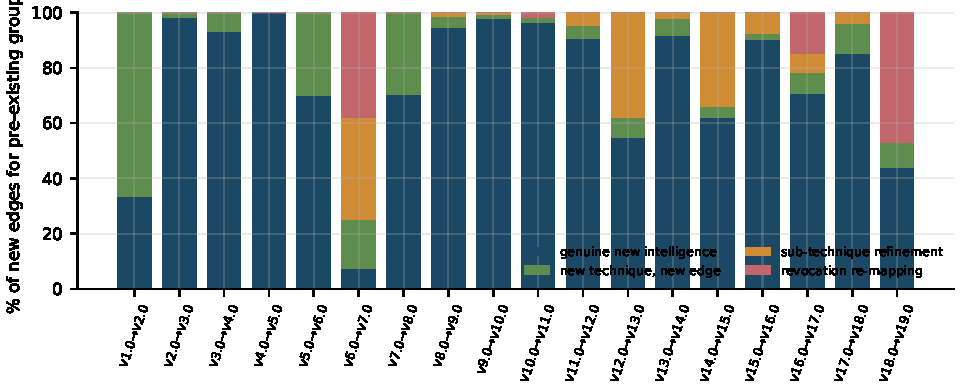
\includegraphics[width=\linewidth]{fig4_growth_decomposition.pdf}
\caption{Per-transition decomposition of new group-technique edges for pre-existing groups.}
\label{fig:4}
\end{figure}


\textbf{Table 5.} Knowledge-growth decomposition, Enterprise. Edges for groups newly added to ATT\&CK are excluded from the denominator; bookkeeping share is refinement plus re-mapping over all new edges for pre-existing groups. Per-transition rows are plotted in Figure 4 and tabulated in full in the reproduction package.

\begin{center}\footnotesize
\begin{tabular}{lllllll}
\toprule
Transition & New edges (pre-existing groups) & Genuine new intel & New technique & Sub-technique refinement & Revocation re-mapping & Bookkeeping share \\
\midrule
v6.0→v7.0 & 1059 & 78 & 187 & 390 & 404 & 0.750 \\
v12.0→v13.0 & 71 & 39 & 5 & 27 & 0 & 0.380 \\
v14.0→v15.0 & 100 & 62 & 4 & 34 & 0 & 0.340 \\
v18.0→v19.0 & 164 & 72 & 15 & 0 & 77 & 0.470 \\
\textbf{All transitions} & \textbf{3074} & \textbf{1752} & \textbf{330} & \textbf{487} & \textbf{505} & \textbf{0.323} \\
\bottomrule
\end{tabular}
\end{center}

Across all Enterprise transitions 5,516 group-technique edges are added, of which 2,442 belong to groups newly added to ATT\&CK. Of the remaining 3,074, 1,752 are genuine new intelligence about a pre-existing pairing, 330 credit a group with a newly minted technique, 487 are sub-technique refinements of an edge the group already had, and 505 restate an edge whose technique was revoked and replaced: a bookkeeping share of 992/3074 = 0.323. The headline conceals a heavy tail, and the tail is the point. The restructuring transition is 0.750 bookkeeping over 1,059 edges and eight transitions are below 0.05, but v12.0 to v13.0 is 0.380 over 71 edges, v14.0 to v15.0 is 0.340 over 100, and the most recent transition is 0.470 over 164 edges, the highest share since the restructuring and driven entirely by 77 revocation re-mappings. A reader who plots ATT\&CK's edge count as a curve of accumulating adversary knowledge is reading a curve that is roughly a third bookkeeping overall and nearly half bookkeeping in the release that shipped four months before this analysis. Evidence from the benchmark side agrees: the 4.3x label-space growth between one LLM CTI benchmark generation and its successor is roughly 96\% pre-existing catalogue, with six genuinely new entries [6].

\subsection{6.5 Recurrence: a hazard, not a wound}

The episodic reading has one defence left, that the 2020 restructuring was singular and is finished. Extending the measurement to all three domains refutes it. Five major transitions have identifier Jaccard below 0.80: Mobile v2.0 to v3.0 (J = 0.000), Enterprise v6.0 to v7.0 (0.222), ICS v8.0 to v9.0 (0.778), Mobile v10.0 to v11.3 (0.268) and ICS v18.0 to v19.0 (0.698). That is 5 events in 47 transitions, a hazard of 0.106 per major transition, one event per 4.41 domain-years over 22.05 observed domain-years, roughly one restructuring somewhere in ATT\&CK every 1.5 calendar years. Two matter more than their Jaccard suggests. Mobile's 2018 event is the most destructive in the corpus and predates the Enterprise restructuring: all 128 STIX identifiers are preserved while all 76 ATT\&CK identifiers vanish, zero of them recoverable, making it invisible to STIX-keyed tooling and uncrosswalkable by any mechanism MITRE publishes. And the ICS event is happening now, introducing sub-techniques for the first time — 0 at v18.1, 18 at v19.0 — six years after Enterprise made the same move, with all nine remaps recoverable. The two clocks are therefore not a story about one bad year: the referential clock is episodic and recurrent across domains, and the intensional clock never stopped.

\textbf{Figure 9.} The two clocks: the intensional clock measured at a common two-year horizon per cohort, and the five restructuring events across the three domains.

\begin{figure}[htbp]
\centering
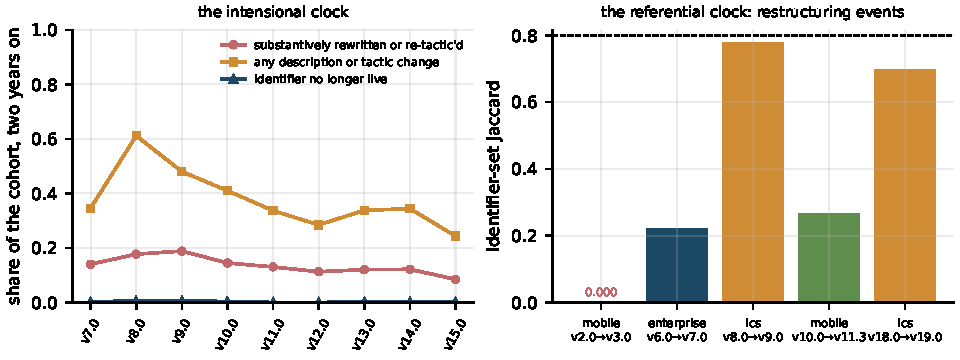
\includegraphics[width=\linewidth]{fig9_two_clocks.pdf}
\caption{The two clocks: the intensional clock at a common two-year horizon per cohort, and the five restructuring events across the three domains.}
\label{fig:9}
\end{figure}


Can a consumer see one coming? Over 17 lagged Enterprise pairs, by Spearman correlation with permutation tests, the largest coefficient is detection-field edits at ρ = +0.429, p = 0.087, with description edits at +0.238 and tactic changes at −0.032; the largest anywhere in the three-domain panel, ICS renames at ρ = +0.733, has p = 0.054 on n = 10. Technique-level hazard modelling is worse than null: the 131 techniques doomed at v7.0 had been edited \emph{less} than the survivors in the preceding release, on description edits (0.168 against 0.336) and version bumps (0.176 against 0.372). Restructuring waves are not forecastable from the public bundles, which removes the option of a triggered response and means any protocol that helps must be standing rather than event-driven. The most recent wave shows what standing exposure looks like: 17 live techniques revoked between v18.1 and v19.2, a blast radius on the v18.1 graph of 84 group-technique edges, 155 software-technique edges, 47 mitigations and 17 detection relationships, 52 of 168 group profiles losing at least one identifier, and T1562.001 ranked 33 of 599 techniques by \texttt{uses} edges in the release it left.

\end{abstract}
\section{Downstream Impact of Drift on CTI Analytics}

\subsection{7.1 What the experiments hold fixed}

Section 6 measures the instrument. This section measures what reading it through the wrong edition costs. Every experiment here obeys R1: the adversary intelligence is identical across conditions and only the vocabulary moves. That is what separates this design from a before-and-after comparison, which would confound drift with eight years of genuine intelligence gain. The cost of the design is stated rather than hidden: back-projecting a modern profile into a 2018 vocabulary finds no expression for 389 of 697 modern techniques, and a group profile retains 0.618 of its distinct identifiers; by v18.0 those are 7 of 697 and 0.998. All legacy conditions consume the same reduced observation, so the contrast among them is unaffected; only the oracle sees the full modern draw, which is why the oracle is read as an unreachable ceiling rather than a baseline.

\subsection{7.2 Attribution}

\textbf{Figure 5.} Top-1 attribution accuracy by condition against the v19.0 knowledge base, and the drift penalty with bootstrap confidence bands, by the vocabulary the artefact was written in.

\begin{figure}[htbp]
\centering
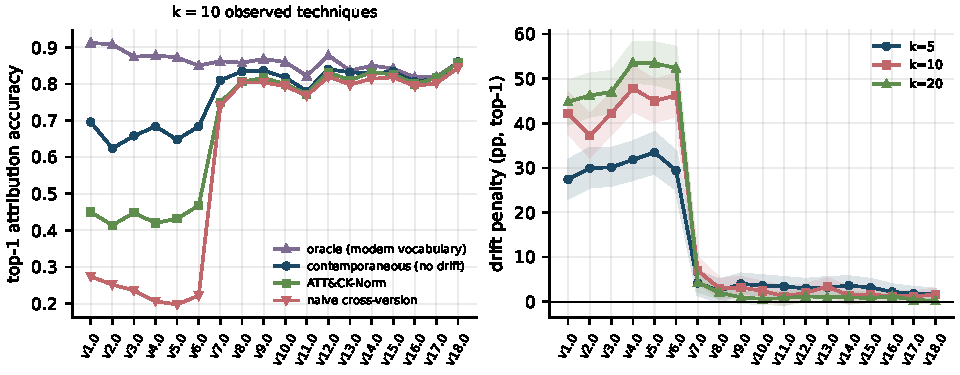
\includegraphics[width=\linewidth]{fig5_attribution.pdf}
\caption{Attribution accuracy by condition, and the drift penalty with bootstrap confidence bands.}
\label{fig:5}
\end{figure}


\textbf{Table 6.} Controlled attribution, k = 10, analysis release v19.0, 500 trials per row, paired bootstrap intervals. Back-projected is the self-consistent legacy system; naive is the same artefact read by the modern base; recovered is the share of the penalty normalization returns.

\begin{center}\footnotesize
\begin{tabular}{lllllllll}
\toprule
Artefact vocabulary & Groups & OOV & Back-projected & Naive & ATT\&CK-Norm & Oracle & Drift penalty (pp) [95\% CI] & Recovered \\
\midrule
v1.0 (2018-01-17) & 47 & 0.256 & 0.696 & 0.274 & 0.450 & 0.912 & 42.2 [37.8, 46.8] & 0.42 \\
v4.0 (2019-04-30) & 70 & 0.264 & 0.684 & 0.206 & 0.420 & 0.878 & 47.8 [42.8, 52.6] & 0.45 \\
v6.0 (2019-10-23) & 78 & 0.283 & 0.684 & 0.222 & 0.468 & 0.850 & 46.2 [41.6, 51.0] & 0.53 \\
v7.0 (2020-03-31) & 88 & 0.013 & 0.810 & 0.740 & 0.750 & 0.862 & 7.0 [4.4, 9.8] & 0.14 \\
v9.0 (2021-04-29) & 102 & 0.016 & 0.836 & 0.804 & 0.816 & 0.868 & 3.2 [1.2, 5.4] & 0.38 \\
v12.0 (2022-10-25) & 123 & 0.011 & 0.840 & 0.820 & 0.832 & 0.878 & 2.0 [0.6, 3.8] & 0.60 \\
v15.0 (2024-04-23) & 138 & 0.013 & 0.834 & 0.818 & 0.826 & 0.842 & 1.6 [0.4, 3.0] & 0.50 \\
v18.0 (2025-10-28) & 161 & 0.015 & 0.860 & 0.844 & 0.858 & 0.858 & 1.6 [0.6, 2.8] & 0.88 \\
\bottomrule
\end{tabular}
\end{center}

The shape is the two-clock structure again, read through a task. An artefact written in the pre-restructuring vocabulary loses 37 to 48 points of top-1 accuracy purely because its identifiers no longer denote, with intervals excluding zero by a wide margin; the same artefact written one release ago loses 1.6 points. Every legacy row has an out-of-vocabulary rate near 0.26 and every modern row near 0.014, and the unresolvable rate — identifiers that survive transitive closure and still fail to land live — is 0.000 in every row. Nothing here is a broken crosswalk. The penalty arises because the crosswalk is applied to a coarse vocabulary, so what it returns is correct and less discriminative than what a modern analyst would have written, which is exactly the O4 defect priced.

The modern penalties are small and they are not zero, which matters because the field's implicit position is that they are zero. Eleven of the twelve post-restructuring rows have intervals excluding zero at k = 10, and the effect is directional in all of them.

\subsection{7.3 Separability and additivity}

R2 requires a noise model rather than a noise-free measurement presented as if it were general. The strongest objection to everything above is that products pinned to a single release already disagree about the label for the same behaviour [74], a noise floor larger than most of the modern penalties. Our design holds the labelling process constant across conditions, so that noise cancels in the contrasts; but a contrast in which a nuisance term is fixed at zero establishes separability, not additivity.

We therefore repeat the experiment with labeller noise injected before back-projection, so it flows into all conditions: with probability ρ an observed technique is replaced by something the same labeller could plausibly have written — a sibling sub-technique, its parent, or another technique in the same tactic, which is the confusion structure reported for real extractors [20]. At ρ = 0.4 the v1.0 penalty falls from 43.9 to 32.0 points and the v6.0 penalty from 47.6 to 30.8, while the v12.0 and v18.0 penalties are unchanged within noise at 1.6 and 1.5 points. Drift survives realistic labeller disagreement at every boundary tested, and it is sub-additive with it where drift is large. The consequence for how the paper should be read is direct: the noise-free figures in Table 6 are upper bounds on what a real analyst pipeline would experience, and we report them as such. Normalization degrades faster than the penalty does — recovery at v1.0 falls from 0.44 to 0.34 as ρ goes from 0 to 0.4 — so the remedy is worth less under realistic noise than under ideal conditions, which is the opposite of the direction a paper advocating its own protocol would prefer.

The archival control corrects a second thing. The self-consistent condition is built by back-projection, and a real archival system is not the same object: judging the actual v1.0 profiles against themselves scores 0.969, against the back-projection's 0.668, because a back-projected profile collides distinct behaviours onto shared coarse identifiers. The two converge by v18.0 at 0.846 and 0.841. The back-projected control is therefore conservative for legacy rows, and the released results files label that condition \texttt{contemporaneous}, which overstates it; we use back-projected throughout and report both.

\subsection{7.4 Where the modern effect lands}

An aggregate of 1.6 points averaged over 161 groups would be easy to dismiss, and the second published objection says why: roughly a third of ATT\&CK groups have no technique unique to them, so most of the population was never attributable [59]. Our corpus reproduces that independently — the share of groups with at least one unique technique is 0.325 at v12.0, 0.309 at v16.0 and 0.298 at v18.0 — and stratifying by it inverts the objection. At v18.0 the drift penalty is +0.0239 [+0.0109, +0.0391] on groups that have a unique technique and +0.0067 [+0.0019, +0.0125] on those that do not; at v12.0, +0.0344 [+0.0101, +0.0587] against +0.0089 [−0.0010, +0.0199]; at v16.0, +0.0331 against +0.0049. Drift bites two-and-a-half to seven times harder on exactly the groups where attribution is possible at all. A small average over a mostly non-identifiable population conceals a material effect on the subset that carries the task.

\subsection{7.5 Conclusions move, not just scores}

Gene Ontology set the bar for this class of claim: showing that scores shift is weaker than showing that conclusions shift [69]. Read at verdict level, an artefact in the v1.0 vocabulary has its named actor changed by the modern knowledge base in 0.722 of observations, and in 0.712 the new name is wrong; at v6.0, 0.790 and 0.774. Across a single modern release boundary, v18.0 to v19.0, the named actor still changes in 0.022 of observations and is wrong in 0.022 of them. Normalization is itself a verdict-changing operation, altering the named actor in 0.368 of v1.0 trials and 0.442 of v6.0 trials, which is why applying it silently inside a pipeline is an integrity event rather than a maintenance step.

\textbf{Figure 8.} Attribution verdict instability by artefact vocabulary, and Kendall tau of the mitigation coverage leaderboard against its original ordering.

\begin{figure}[htbp]
\centering
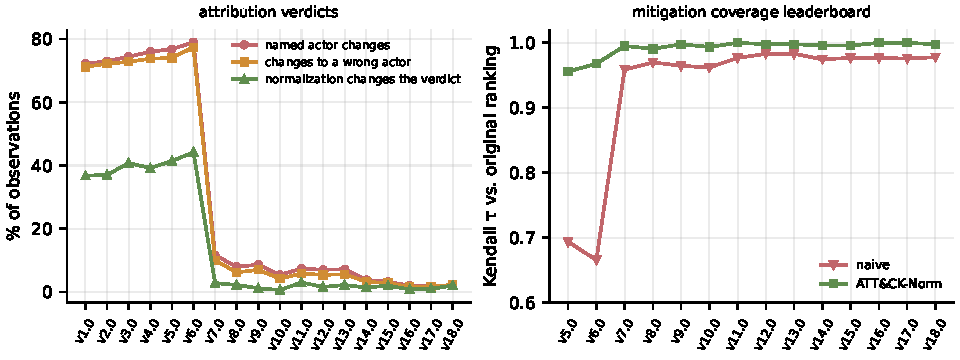
\includegraphics[width=\linewidth]{fig8_conclusion_flips.pdf}
\caption{Attribution verdict instability, and mitigation leaderboard reordering.}
\label{fig:8}
\end{figure}


The same instability reaches rankings. Freezing every mitigation's technique portfolio at a release and re-ranking the mitigations at v19.0 — the portfolios unchanged, only the vocabulary moving — gives Kendall tau against the original ranking of 0.694 at v5.0 and 0.665 at v6.0, restored to 0.956 and 0.968 by normalization. Modern tau is high but not one: 0.976 at v17.0 and 0.978 at v18.0, and at both of those the top-ranked mitigation changes identity under naive matching while normalization holds it in place. A leaderboard whose first place moves because the catalogue was re-edited is a leaderboard reporting something other than what its caption claims.

\subsection{7.6 Coverage claims}

\textbf{Figure 6.} Reported coverage under a capability frozen at each release and re-measured at v19.0, naively and after normalization, with a 500-sample random-portfolio sweep.

\begin{figure}[htbp]
\centering
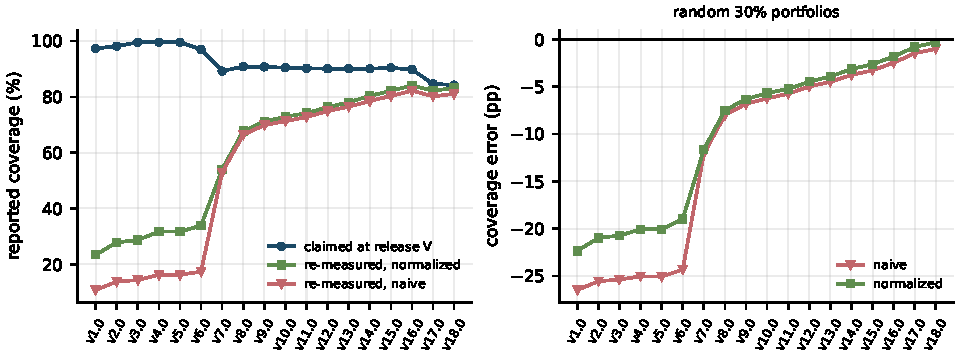
\includegraphics[width=\linewidth]{fig6_coverage.pdf}
\caption{Reported coverage under a frozen capability, and the random-portfolio sweep.}
\label{fig:6}
\end{figure}


A capability frozen at v6.0 claimed 97.0\% coverage at the time and reads 17.4\% at v19.0; frozen at v10.0, 90.5\% reads 71.3\%; at v17.0, 84.7\% reads 80.2\%; at v18.0, 84.2\% reads 81.1\%. Most of that fall is not artefact. A growing denominator is O1 doing exactly what it should: the technique catalogue grew and the frozen capability genuinely covers less of it. The artefact is the gap between naive and normalized re-measurement, which isolates identifiers the capability still covers but can no longer match: 16.5 points at v6.0, 1.6 at v10.0, 2.0 at v17.0 and 2.1 at v18.0, with a 500-sample random-portfolio sweep giving the same shape. Two to three points of a published coverage number that is nothing but identifier arithmetic is not a rounding error in a market where products are compared on such numbers [80, 82, 84], and it sits on top of a denominator that other work argues is the wrong unit entirely [62, 64] and a ceiling set by the control catalogue rather than the product [58].

The long-tail objection applies here and fails on measurement. If drift landed only on rarely used techniques, a prevalence-weighted number would barely move. Weighting each technique by the \texttt{uses} edges the release itself publishes makes the artefact larger, not smaller: 20.0 points against 16.5 at v6.0, and 1.57 against 2.15 at v18.0, with the fifteen most-referenced techniques carrying 0.285 of all edges. The v19 wave took T1562.001 at rank 33 of 599. The weight here is documentation prevalence, not telemetry prevalence, and Section 11 states what that does not settle.

\end{abstract}
\section{ATT\&CK-Norm: A Version-Normalization Protocol}

\subsection{8.1 The protocol, and what it returns}

ATT\&CK-Norm maps an identifier set onto a target release: transitive \texttt{revoked-by} closure, cycle-safe and bounded at ten hops; identifiers that are deprecated or absent at the target are dropped and counted; and the result is not a set but a ledger of what was kept, what was merged and by how much, what changed abstraction level, and what was dropped. The ledger is the contribution, not the mapping. A protocol returning only the projected set silently destroys the information a reader needs, which is the reporting failure this paper is about, committed by the paper's own remedy.

Measured on this corpus it is worth having and worth distrusting. It recovers 0.42 to 0.53 of the attribution penalty on pre-restructuring artefacts and moves mitigation-ranking tau from 0.665 to 0.968 at v6.0, removing every rank-1 flip in the corpus and introducing none. On post-restructuring artefacts it recovers a fraction of a penalty that is already small, and its gain interval spans zero in most modern conditions. It is a legacy migration tool. Anything claiming it is a standing cure for drift is claiming something this measurement contradicts.

\subsection{8.2 Six defects, measured}

First, \textbf{merges destroy cardinality}. Eight Enterprise targets absorb 20 predecessors and T1685 absorbs five, so a set-returning normalizer collapses distinct assertions into one and reports success. On real corpora that is 537 distinct classes reduced to 503 for the TRAM bootstrap corpus, with 0.1475 of its 25,770 label instances landing in a merged class, and 215 reduced to 199 for rcATT, with 0.0937 of its 6,235 instances.

Second, \textbf{the official crosswalk demotes abstraction}. Of the 149 Enterprise revocation edges, 119 map a top-level technique onto a sub-technique and 7 do the reverse. Normalization follows them and reports a clean result; on rcATT, 88 of its resolutions change abstraction level and 28 do so for the TRAM corpus.

Third, \textbf{it is blind to intension}. Between v18.1 and v19.2, 674 techniques are live and identifier-stable, of which 198 changed tactic and 41 changed description. The protocol returns all 674 unchanged, signalling zero drift on the release that dissolved Defense Evasion.

Fourth, \textbf{cross-layer promotion is not representable}. No tactic object in the corpus carries a revocation edge, so the promotion of T1562's concept to the tactic layer has no expression the protocol can follow.

Fifth, \textbf{the roll-up branch is dead}. Climbing to a surviving parent when an identifier has no successor fires 3 times in 12,027 resolutions across every domain and major release, because ATT\&CK does not orphan sub-techniques in practice. It was the only path that could fabricate a parent-level assertion the artefact never made, and it bought nothing, so it is off by default and the honest default is drop-and-count.

Sixth, \textbf{it has no domain guard}, which Section 9 shows is not hypothetical.

\subsection{8.3 Two worked counter-examples}

\texttt{normalize(\{T1562\})} against v19.2 returns \texttt{\{T1685\}} in one hop, drops nothing, and reports success. T1562 was \emph{Impair Defenses}, the parent of twelve children; T1685 is \emph{Disable or Modify Tools}, which was one of those children. The protocol has silently replaced an assertion about a family with an assertion about one member of it, and nothing in the ledger's kept column distinguishes that from an exact successor — only the abstraction-change flag does, which is why the flag exists.

The second counter-example is worse because it is a false positive. Of CTIBench's eight labels invalid at v19.2, seven come from one row whose platform column reads Enterprise while its gold set is entirely Mobile identifiers, all seven live in Mobile v19.2. A domain-unaware protocol reports seven unrepairable deprecations; the truth is one mis-typed row. That is 0.875 of the apparent drift damage in that corpus being a labelling error the protocol would have confidently misdiagnosed, and it is the clearest argument for a residual ledger a human reads rather than a number a pipeline consumes [4, 30].

\end{abstract}
\section{Label Validity of Deployed CTI Corpora}

\textbf{Figure 7.} Share of each corpus's distinct labels that are live, evaluated at every published ATT\&CK release.

\begin{figure}[htbp]
\centering
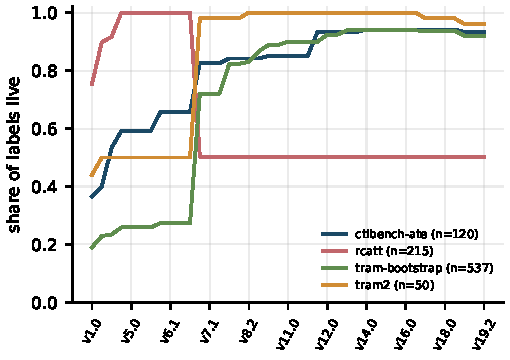
\includegraphics[width=\linewidth]{fig7_artifact_validity.pdf}
\caption{Label-validity curves for four deployed CTI corpora.}
\label{fig:7}
\end{figure}


\textbf{Table 9.} Label validity of four deployed CTI corpora, evaluated per declared domain against every published release. A corpus with no consistent release mixes identifiers from mutually exclusive vocabularies.

\begin{center}\footnotesize
\begin{tabular}{lllllllll}
\toprule
Corpus & Distinct labels & Label instances & Sub-technique labels & Best-fit release & Fit & Releases where all labels valid & Invalid today & Repairable \\
\midrule
CTIBench CTI-ATE & 120 & 397 & 0 & v14.0 (2023-10-31) & 0.942 & \textbf{none} & 8 (0.067) & 1 \\
rcATT & 215 & 6235 & 0 & v4.0 (2019-04-30) & 1.000 & 8 (v4.0–v6.3) & 107 (0.498) & 99 \\
TRAM bootstrap & 537 & 25770 & 344 & v13.0 (2023-04-25) & 0.939 & \textbf{none} & 43 (0.080) & 43 \\
TRAM 2 & 50 & 5143 & 24 & v8.2 (2021-01-27) & 1.000 & 18 (v8.2–v16.1) & 2 (0.040) & 2 \\
\bottomrule
\end{tabular}
\end{center}

Two of the four corpora can be dated precisely from their labels alone, which is itself a useful capability: rcATT's vocabulary is simultaneously live only across v4.0 to v6.3 and TRAM 2's only across v8.2 to v16.1, so an undeclared artefact's release can be bounded by inspection [8, 10], the same move AVClass makes for malware family aliases [19]. Two cannot be dated at all, because no release makes every label simultaneously valid — the corpus mixes vocabularies. For the CTIBench extraction task that mixture is the mis-typed row of Section 8.3; for the TRAM bootstrap corpus it is a wider spread that the corpus's own documentation does not resolve, and two independent 2026 efforts decline to treat its annotations as gold at all [52, 73]. Decay is severe where the artefact is old and the field keeps citing it anyway: 0.498 of rcATT's distinct labels and 0.380 of its label instances are invalid today, in a corpus still used as a baseline [8, 44]. The successor generation's answer to staleness is to rebuild from live APIs rather than to declare a release [13], which trades an undeclared pin for no pin at all.

The adoption evidence is what makes this a systemic finding rather than four case studies. A documentation scan of the three corpora's own repositories finds zero ATT\&CK version declarations across 19 files (Table 12). Extending the scan to published coverage artefacts: across 69 ATT\&CK Navigator layer files in the cloned public repositories, 5 declare an ATT\&CK release and all five carry the same value; the 69 layers hold 4,821 technique annotations of which 917 (0.190) are not live at v19.2, with 60 of the 69 layers carrying at least one dead annotation and 818 of the 917 recoverable by crosswalk. The Navigator's own layer format makes the field optional and silently defaults a version-less layer to the current release [15, 16], and the most widely used third-party generator omits it unless asked [79]. So the mechanism that would repair four-fifths of the damage exists, is documented, and is not used.

\end{abstract}
\section{Discussion and Reporting Discipline for CTI Research}

The remedy is not a better crosswalk. Section 8 is a crosswalk being pushed to its limit and failing in ways a better crosswalk does not fix, because the failures are semantic and the crosswalk is referential. What is missing is a reporting discipline, and it is four lines a reviewer can check.

\textbf{One.} The artefact declares its ATT\&CK domain, the exact release, and the bundle hash. Release alone is insufficient where point releases exist and the Navigator truncates them.
\textbf{Two.} If identifiers were normalized, the artefact declares the target release.
\textbf{Three.} The artefact publishes the residual: how many identifiers were kept, merged, demoted across abstraction levels, and dropped. A normalization reporting only the survivors is not reproducible.
\textbf{Four.} Any comparison across time states the common reference release both sides were projected onto, or states that no projection was done.

Two addenda follow from the measurements. A benchmark also declares its granularity policy — whether sub-technique identifiers are permitted, and whether a parent-level answer scores against a sub-technique gold label — because two benchmarks with the same task name and different policies produce numbers with no arithmetic relation. A vendor coverage claim also publishes the denominator's cardinality and the release it came from, since the denominator moves on its own (Section 7.6). The cost is honest: rcATT's residual line would read that half its vocabulary is invalid, and that is precisely the information a reader needs.

For CTI quality frameworks the finding is a missing dimension. The canonical dimension sets cover accuracy, timeliness, completeness, relevance, provenance and interoperability [60, 76], and provenance there means who produced the intelligence, not which edition of the reference vocabulary it is written in. We propose \textbf{vocabulary provenance} as a distinct dimension, with the four lines above as its instrument, alongside the dynamic-assessment machinery that literature already builds [27, 41]. It is testable mechanically, unlike most quality dimensions in that literature, which is an argument for it rather than against.

For MITRE the proposals are ports, not inventions, and each has a measurement behind it. An inexact-successor relation alongside \texttt{revoked-by}, so a re-cut is distinguishable from an exact replacement [54, 26] — 119 of 149 edges need it. A controlled obsolescence-reason vocabulary and label-level visibility of obsoletion [54]. Referent stability enforced: TA0005 should have been retired and a new identifier minted rather than renamed in place [53, 54]. \texttt{priorVersion} and \texttt{backwardCompatibleWith} links between releases [57]. A typed evolution mapping published as an artefact, which is what COnto-Diff means by an evolution mapping and what ATT\&CK Sync stops short of [26, 5], and which the knowledge-graph literature already tracks as a time series in its own right [37]. A change signal for intension, since the present one operates at precision 0.447. And a mandatory version field in the Navigator layer format, which would convert 64 of 69 published layers from undated to dated at no cost to their authors.

\end{abstract}
\section{Threats to Validity}

R3 requires a declared closure boundary, and the most important one is that this study is computed inside a single curator's graph. Observations, candidate profiles, ground truth and the back-projection map all derive from ATT\&CK's own edges. The absolute accuracies in Table 6 are therefore internal-consistency scores and not attribution performance, and we do not present them as the latter. The contrasts are the result; the levels are scaffolding. The experiment that would close this boundary does not exist publicly: a double-labelled incident corpus in which two analysts label the same intrusions under two releases, yielding the drift term and the labeller-noise term simultaneously and from outside MITRE's edges.

Three narrower limits. The back-projection is a synthetic transcription and Section 7.3 gives its bias direction and magnitude. The naive condition is a uniform worst case — a real artefact mixes granularities, so a real pipeline sits between naive and back-projected rather than at naive. And the prevalence weighting of Section 7.6 uses documented \texttt{uses} edges, a cumulative documentation stock drawn from the same release whose churn is being measured; the long-tail objection is refuted for the written CTI corpus and untested for the alert stream, which would need telemetry we cannot reach.

On evidence, three tiers are marked throughout and the second is the weak one. Tier A claims are computed from artefacts read in full and are reproducible. Tier B claims are secondary literature reached only through search summaries in this environment; they are attributed as reported and never quoted, and no numeric claim from a Tier B source is load-bearing for any finding. Tier C is the audited absence of Section 3, stated with its search bound rather than as proof.

One process disclosure belongs here because the alternative is to conceal it. The literature corpus was assembled by parallel agents, and an integrity check of all 112 notes found 10 whose front matter and body described different sources — a provenance failure of exactly the kind this paper studies, inside the paper's own evidence base. All ten were quarantined and excluded from the reference registry, none is cited, and the claims that had rested on them were re-derived from artefacts read directly: the revocation-arity and tactic-layer results in Section 6.2 are recomputed from the release bundles, and MITRE's change taxonomy and ATT\&CK Sync's outputs were re-read from their repositories [34, 5].

R4 requires a named falsifier, in the spirit of the pitfall catalogues that made temporal hygiene checkable [35, 67], and there are two. The measurement's temporal model fails if substantive-rewrite rates fall below about 3\% per year across all three domains for three consecutive major releases, or if no domain records an identifier Jaccard below 0.80 in the next eight domain-years. The paper's thesis fails if a representative sample of published CTI artefacts turns out to carry resolvable release pins in the majority \emph{and} mechanical forward migration from those pins reproduces an independently authored current-version mapping to within inter-analyst agreement. On the evidence of Section 9 — 5 of 69 layers dated, zero of 19 documentation files — the first conjunct is not close to true today, but it is the right test and it is a test someone could run.

\end{abstract}
\section{Conclusion}

ATT\&CK is a measuring instrument that has been re-issued 109 times without any downstream result recording which issue it used. Its identifier accounting is sound, complete for Enterprise, and almost never used: 5 of 69 published coverage layers declare a release, and 0.190 of their annotations no longer denote. Its semantic accounting does not exist, and cannot be inferred from the metadata it publishes, whose change signal runs at precision 0.447 and recall 0.641. The consequences reach conclusions rather than scores — the named actor, the top-ranked mitigation, the pass or fail of a benchmark item — and they are concentrated on exactly the cases where the analytic was doing real work.

Identifier normalization repairs the referential half, and we have spent a section arguing against treating it as the contribution: it recovers roughly half the legacy attribution penalty, buys under a point on modern artefacts, collapses five identifiers into one unannounced, demotes an abstraction level in 119 of 149 edges, and returns a clean bill of health on the release that dissolved a tactic. Identifier arithmetic buys comparability of identifiers. It buys nothing about whether two identifiers mean the same thing. What remains is governance, and it is four lines in an artefact header plus seven ports from an ontology-engineering literature that settled these questions decades ago. The field's habit of citing ATT\&CK where it should be pinning it is not notational sloppiness; it is why a measurable, recurrent and largely unsignalled source of invalidity has gone unmeasured until now.

\end{abstract}
\section{Sources}

Entries are numbered as in this study's reference registry; only entries
cited in the text are listed. Sources marked as read in full were obtained
from local clones of the named repositories; the remainder were reachable
in this environment only through search summaries and are attributed as
reported rather than quoted.

1. ATT\&CK's published retirement contract, read from the artefact. https://github.com/mitre-attack/attack-stix-data/blob/master/USAGE.md
2. AttacKG repo audit: ATT\&CK ontology frozen as a 2021-08-31 HTML scrape, parent-only…. https://github.com/li-zhenyuan/Knowledge-enhanced-Attack-Graph
3. B2 synthesis: six TTP systems, five different ATT\&CK ontologies, two declared versions. https://github.com/center-for-threat-informed-defense/tram
4. CTI-Bench data audit: v15-era vocabulary hard-coded into prompts, sub-techniques erased…. https://github.com/maveryn/cti-bench
5. CTID ATT\&CK Sync: what it publishes, read from the repository. https://github.com/center-for-threat-informed-defense/attack-sync
6. Measured: 4.3x label-space growth between CTIBench and AthenaBench is \textasciitilde{}96\% pre-existing…. https://github.com/Athena-Software-Group/athenabench
7. MITRE's own change taxonomy, read from diffStix source. https://github.com/mitre-attack/mitreattack-python
8. rcATT repo audit: a 2019-era flat ATT\&CK label space, half of it revoked by v13. https://github.com/vlegoy/rcATT
10. tumeteor/mitre-ttp-mapping audit: a declared v12.0 remap that still leaks pre-v7 revoked…. https://github.com/tumeteor/mitre-ttp-mapping
11. A Comprehensive Survey of Threat Intelligence Research: A Measurement-Based Study (ACM…. https://dl.acm.org/doi/10.1145/3772280
12. APT attribution survey (JISA 2025): taxonomy by artefact type, not by ontology version. https://doi.org/10.1016/j.jisa.2025.104076
13. AthenaBench (arXiv 2511.01144): dynamic live-API benchmarking as the field's answer to…. https://arxiv.org/abs/2511.01144
14. ATT\&CK Design and Philosophy: inclusion criteria are explicitly non-stationary and…. https://attack.mitre.org/docs/ATTACK\_Design\_and\_Philosophy\_March\_2020.pdf
15. ATT\&CK Navigator layer file format: the ATT\&CK content version is an optional field that…. https://github.com/mitre-attack/attack-navigator/blob/master/layers/spec/v4.5/layerformat.md
16. ATT\&CK Navigator layer upgrade: version stamping is mandatory, migration is manual…. https://github.com/mitre-attack/attack-navigator/blob/master/USAGE.md
17. AttackSeqBench (arXiv 2503.03170): sequence-level ATT\&CK reasoning and the…. https://arxiv.org/abs/2503.03170
19. AVClass: alias resolution and label normalization as prior art for a migration map. https://software.imdea.org/\textasciitilde{}juanca/papers/avclass\_raid16.pdf
20. Beyond Single Reports — intra-version technique confusability as a rival explanation for…. https://arxiv.org/abs/2604.07470
21. Boundary synthesis: where concept-drift literature stops and ontology drift begins.
22. CADE: Detecting and Explaining Concept Drift Samples for Security Applications. https://www.usenix.org/conference/usenixsecurity21/presentation/yang-limin
23. CAPTAIN / Chasing the Shadows: TTP-sequence attribution with no declared ATT\&CK version. https://arxiv.org/abs/2409.16400
24. Class-Incremental Learning surveys: the additive quadrant of label-space change. https://arxiv.org/abs/2302.03648
25. Cleaning the NVD and the security knowledge-base data-quality genre. https://arxiv.org/pdf/2006.15074
26. COnto-Diff (Hartung, Gross, Rahm): complex change operations as evolution mappings…. https://www.sciencedirect.com/science/article/pii/S1532046412000627
27. CTI Quality Assessment Cluster — automated dynamic assessment, MISP weighted criteria…. https://www.sciencedirect.com/science/article/pii/S0167404824003845
28. CTI-REALM (arXiv 2603.13517): telemetry-grounded detection evaluation as the only…. https://arxiv.org/abs/2603.13517
29. CTIArena to CTIConnect (arXiv 2510.11974): 691 to 1,860 QA pairs under one identifier…. https://arxiv.org/abs/2510.11974
30. CTIBench (NeurIPS 2024): authoritative-source design treats ATT\&CK as fixed, has a…. https://proceedings.neurips.cc/paper\_files/paper/2024/file/5acd3c628aa1819fbf07c39ef73e7285-Paper-Datasets\_and\_Benchmarks\_Track.pdf
31. CVE identifier lifecycle: REJECTED, DISPUTED, merge and split as security-vocabulary…. https://www.cve.org/Resources/Media/Archives/OldWebsite/about/faqs.html
32. CVE-CWE-CPE mapping instability: abstraction-ladder drift between security vocabularies. https://dl.acm.org/doi/10.1145/3641819
33. Dataset shift and concept drift taxonomies (Gama, Moreno-Torres, Lu et al.). https://dl.acm.org/doi/10.1145/2523813
34. diffStix: MITRE's own machine-readable ontology-drift ledger — and the errors it defends…. https://github.com/mitre-attack/mitreattack-python/tree/master/mitreattack/diffStix
35. Dos and Don'ts of Machine Learning in Computer Security (Arp et al.). https://www.usenix.org/conference/usenixsecurity22/presentation/arp
37. Evolution of vocabulary terms in knowledge graphs: vocabulary churn vs instance-data…. https://arxiv.org/pdf/1710.00232
38. FeedMeter — Evaluating the Quality of Community-Driven Threat Intelligence (2024). https://www.scitepress.org/Papers/2024/123576/123576.pdf
39. Fragmentation of CVSS scores in the NVD: cross-version incomparability in a security…. https://www.sciencedirect.com/science/article/abs/pii/S0167404826001549
40. Geras \& Schreck — The Big Beast to Tackle: Practices in Quality Assurance for CTI (RAID…. https://dl.acm.org/doi/10.1145/3678890.3678903
41. Griffioen, Booij \& Doerr — Quality Evaluation of Cyber Threat Intelligence Feeds (ACNS…. https://link.springer.com/chapter/10.1007/978-3-030-57878-7\_14
42. IncreTTP: ATT\&CK version updates framed as concept drift — and why incremental learning…. https://link.springer.com/chapter/10.1007/978-3-032-23450-6\_2
43. LECO: Continual Learning with Evolving Class Ontologies (NeurIPS 2022). https://arxiv.org/abs/2210.04993
44. Legoy et al. 2020 — Automated Retrieval of ATT\&CK Tactics and Techniques (rcATT paper). https://arxiv.org/abs/2004.14322
45. Li et al. — Reading the Tea Leaves: A Comparative Analysis of Threat Intelligence (USENIX…. https://www.usenix.org/conference/usenixsecurity19/presentation/li
46. MITRE ATT\&CK Evaluations: a governed measurement protocol that refuses to emit a coverage…. https://evals.mitre.org/methodology-overview/
47. MITRE ATT\&CK: State of the Art and Way Forward (ACM CSUR 2025) — the novelty bar an SCI…. https://dl.acm.org/doi/10.1145/3687300
48. MITRE diffStix changelog\_helper: ATT\&CK's own change taxonomy, patch detection, and…. https://github.com/mitre-attack/mitreattack-python/blob/master/mitreattack/diffStix/changelog\_helper.py
50. Modern malware drift adaptation (MORPH, ADAPT, few-sample adaptation): still a fixed…. https://arxiv.org/pdf/2401.12790
51. MOTIF: ground-truth malware family labels and the open, unstable class set. https://arxiv.org/abs/2111.15031
52. Multi-label ATT\&CK classification (arXiv 2606.18166): TRAM annotations declared not-gold…. https://arxiv.org/abs/2606.18166
53. OBO Foundry Identifier Policy: global uniqueness, no reuse, and persistence as a provider…. https://obofoundry.org/id-policy.html
54. OBO Foundry Principle 19: Stability of Term Meaning (referent stability, obsoletion…. https://obofoundry.org/principles/fp-019-term-stability.html
55. OBO Foundry Principle 4: Versioning (version IRIs, release immutability, perpetual…. https://obofoundry.org/principles/fp-004-versioning.html
56. Ontology evolution vs ontology versioning: change management as the core task (Klein…. https://www.researchgate.net/publication/37538421\_Change\_Management\_The\_Core\_Task\_of\_Ontology\_Versioning\_and\_Evolution
57. OWL versioning vocabulary: versionIRI, priorVersion, backwardCompatibleWith…. https://www.w3.org/2007/OWL/wiki/Ontology\_Versions
58. Rahman \& Williams (arXiv:2211.06500): mitigation coverage has a ceiling set by the…. https://arxiv.org/abs/2211.06500
59. Saha et al. — Kitten or Panda? Two-thirds of ATT\&CK threat groups have no group-specific…. https://arxiv.org/abs/2506.10645
60. Schlette et al. — Measuring and Visualizing Cyber Threat Intelligence Quality (IJIS 2021). https://link.springer.com/article/10.1007/s10207-020-00490-y
61. SEvenLLM (arXiv 2405.03446): 90k samples and 28 tasks from 8,485 reports spanning…. https://arxiv.org/abs/2405.03446
62. Shen et al. (ASIA CCS 2024): whole-graph re-analysis of MITRE Evaluations shows…. https://arxiv.org/abs/2401.15878
63. SoK: The MITRE ATT\&CK Framework in Research and Practice — non-comparability already…. https://arxiv.org/abs/2304.07411
64. Summiting the Pyramid v5.0 (CTID): implementations replace techniques as the coverage…. https://github.com/center-for-threat-informed-defense/summiting-the-pyramid
65. SynthCTI (arXiv 2507.16852): synthesising the ATT\&CK long tail, and what that says about…. https://arxiv.org/abs/2507.16852
66. Synthetic APTs (2026): LLM agents reproduce documented APT profiles at 55-80\% precision. https://arxiv.org/abs/2606.07158
67. TESSERACT: Eliminating Experimental Bias in Malware Classification across Space and Time. https://arxiv.org/abs/1807.07838
68. The CTI Echo Chamber — vendor fragmentation as the confounder the drift thesis must…. https://arxiv.org/abs/2602.17458
69. Tomczak et al. (2018): Gene Ontology evolution changes the interpretation of biological…. https://www.nature.com/articles/s41598-018-23395-2
70. Transcend and Transcendent: Conformal Evaluation and Rejection under Concept Drift. https://arxiv.org/abs/2010.03856
71. TTPDrill (ACSAC 2017): the pre-sub-technique baseline everyone still compares against. https://dl.acm.org/doi/10.1145/3134600.3134646
72. TTPHunter / TTPXHunter: 50 then 193 TTP classes, no declared ATT\&CK release. https://arxiv.org/abs/2403.03267
73. TTPrint (arXiv 2605.25836): TRAM-Clean fork and verification against official ATT\&CK…. https://arxiv.org/abs/2605.25836
74. Virkud et al. (USENIX Security 2024): ATT\&CK coverage is not comparable across products…. https://www.usenix.org/conference/usenixsecurity24/presentation/virkud
75. When Benchmarks Age: quantifying answer-key decay in static benchmarks. https://arxiv.org/abs/2510.07238
76. Zibak et al. — Threat Intelligence Quality Dimensions for Research and Practice (DTRAP…. https://dl.acm.org/doi/full/10.1145/3484202
77. 'ATT\&CK is an ontology, not a taxonomy' — the definitional defence and the…. https://www.tripwire.com/state-of-security/attck-structure-ontology
78. ATT\&CK v19 retires Defense Evasion: tactic reassignment at scale, and the industry's…. https://medium.com/mitre-attack/attack-v19-ff329cb65d66
79. DeTT\&CT omits the ATT\&CK version from generated Navigator layers by default, and stamps…. https://github.com/rabobank-cdc/DeTTECT
80. Forrester: a 100\% ATT\&CK Evaluations claim is a red flag — selective presentation…. https://www.forrester.com/blogs/dont-trust-vendor-claims-about-getting-100-on-the-mitre-attck-evaluations
81. How coverage layers are actually built: ad hoc scoring schemes over a data-source mapping…. https://blog.reconinfosec.com/automating-coverage-analysis-with-att-ck-navigator
82. Vendor ATT\&CK coverage claims: '100\% of what, exactly?' and the five ways a coverage…. https://www.attackiq.com/2026/03/10/what-does-mitre-attack-coverage-really-mean/
83. VMRay — STIX and TAXII Explained: Why a Valid Feed Still Might Not Be Usable. https://www.vmray.com/stix-taxii-explianed/
84. Practitioner critique: the ATT\&CK heatmap counts rules, not coverage, and three…. https://dev.to/chrisray/your-attck-heatmap-is-counting-rules-not-coverage-2gh3
\end{document}
